\documentclass{article}      % Specifies the document class

%encoding
%--------------------------------------
\usepackage[ddmmyyyy]{datetime}
%--------------------------------------

%encoding
%--------------------------------------
\usepackage[utf8]{inputenc}
\usepackage[T1]{fontenc}
%--------------------------------------

%colors
%--------------------------------------
\usepackage[usenames, dvipsnames]{color}
%--------------------------------------


%images
%--------------------------------------
\usepackage{graphicx}
%--------------------------------------

%Header and footer commands
%--------------------------------------
\usepackage{lastpage}
\usepackage{fancyhdr}
%--------------------------------------

%%%%%%%%%%%%%%%%%%%%%%%%%%%%%%%%%%%%%%%
%ALTERAR AQUI A VERSÃO DO DIGESTOR!!!!!
\newcommand{\versiondigester}{v1.0.0.7}
%%%%%%%%%%%%%%%%%%%%%%%%%%%%%%%%%%%%%%%

%Header and footer commands
%--------------------------------------
\pagestyle{fancy}
\fancyhf{}
\rhead{Digester \versiondigester}
\lhead{Yandeh}
\lfoot{Yandeh}
\rfoot{\today}
\fancyfoot[C]{\footnotesize Página \thepage\ de \pageref{LastPage}}

\fancypagestyle{firststyle}
{
   \fancyhf{}
   \rhead{Digester \versiondigester}
   \lhead{Yandeh}
   \lfoot{Yandeh}
   \cfoot{Página \thepage}
   \rfoot{\today}
   \fancyfoot[C]{\footnotesize Página \thepage\ de \pageref{LastPage}}
}

%Portuguese-specific commands
%--------------------------------------
\usepackage[portuguese]{babel}
%--------------------------------------

%Hyphenation rules
%--------------------------------------
\usepackage{hyphenat}
\hyphenation{mate-mática recu-perar}
%--------------------------------------

\title{Release Notes \\
      Digester \versiondigester}  % Declares the document's title.
\author{Yandeh Team}              % Declares the author's name.
\date{São Paulo, \today}       

\begin{document}             % End of preamble and beginning of text.

\maketitle                   % Produces the title.

\thispagestyle{firststyle}


\begin{table}[!ht]
\centering
\caption{Histórico de atualizações}
\label{my-label}
\begin{tabular}{|l|l|l|l|}
\hline
\textbf{Versão} & \textbf{Data} & \textbf{Descrição}                & \textbf{Autor}                                       \\ \hline
1.0.0.0           & 22/06/2016    & Revisão Inicial                 & Danilo Guanabara                                     \\ \hline
1.0.0.1           & 27/06/2016    & Bugfixes                        & Danilo Guanabara                                     \\ \hline
1.0.0.2           & 30/06/2016    & Bugfixes e limpeza              & Rosemary Sumitani                                    \\ \hline
1.0.0.3           & 04/07/2016    & Testes Unitários, bugfixes      & Danilo e Rosemary                                    \\ \hline
1.0.0.4           & 07/07/2016    & Parser Daruma, Bugfixes         & Luis, Danilo e Rosemary                              \\ \hline
1.0.0.5           & 17/07/2016    & Bugfixes Parser Daruma          & Luis Sant'Ana                                        \\ \hline
1.0.0.6           & 14/07/2016    & BugFixes Parser Daruma          & Luis Sant'Ana                                        \\ \hline  
1.0.0.7           & 18/07/2016    & BugFixes Troca Impressoras      & Luis e Danilo                                        \\ \hline  
\end{tabular}
\end{table}



\section{Objetivos}

Este documento tem o objetivo de descrever as alterações nas funcionalidades do Digester para a versão \versiondigester. 


\section{Introdução}     
Nesta versão foi corrigido problemas encontrados quando trocamos de impressoras.

\section{O que mudou?}

Nenhuma novidade em relação à versão anterior, apenas correções de \emph{bugs}.

\subsection{Bug fixes}
\begin{itemize}
    \item \colorbox{BurntOrange}{COO errado para Epson}. Problema relacionado ao processo de coleta. 
    \item Não coleta Bematech. Não estava trocando de impressora, porque não estava sendo chamado o parser correto de cada impressora.
    \item Uma mudança da impressora Sweda para a impressora Epson não foi realizada, porém mostra que foi. Resolvida com a alteração do item anterior, mesmo assim este problema não tem impacto na qualidade dos dados.
\end{itemize}


\section{Limitações}
Nenhuma limitação a princípio.

\section{Como funciona?}

Dentro da estrutura de arquivos (/home/hadoop/Coleta/) existe um arquivo chamado $processa\_genericos.py$, onde pode ser editado o seguinte trecho em amarelo, indicando a faixa de dias a serem processados e o trecho em verde indica o ano e mês.

\begin{figure}[!ht]
  \centering
    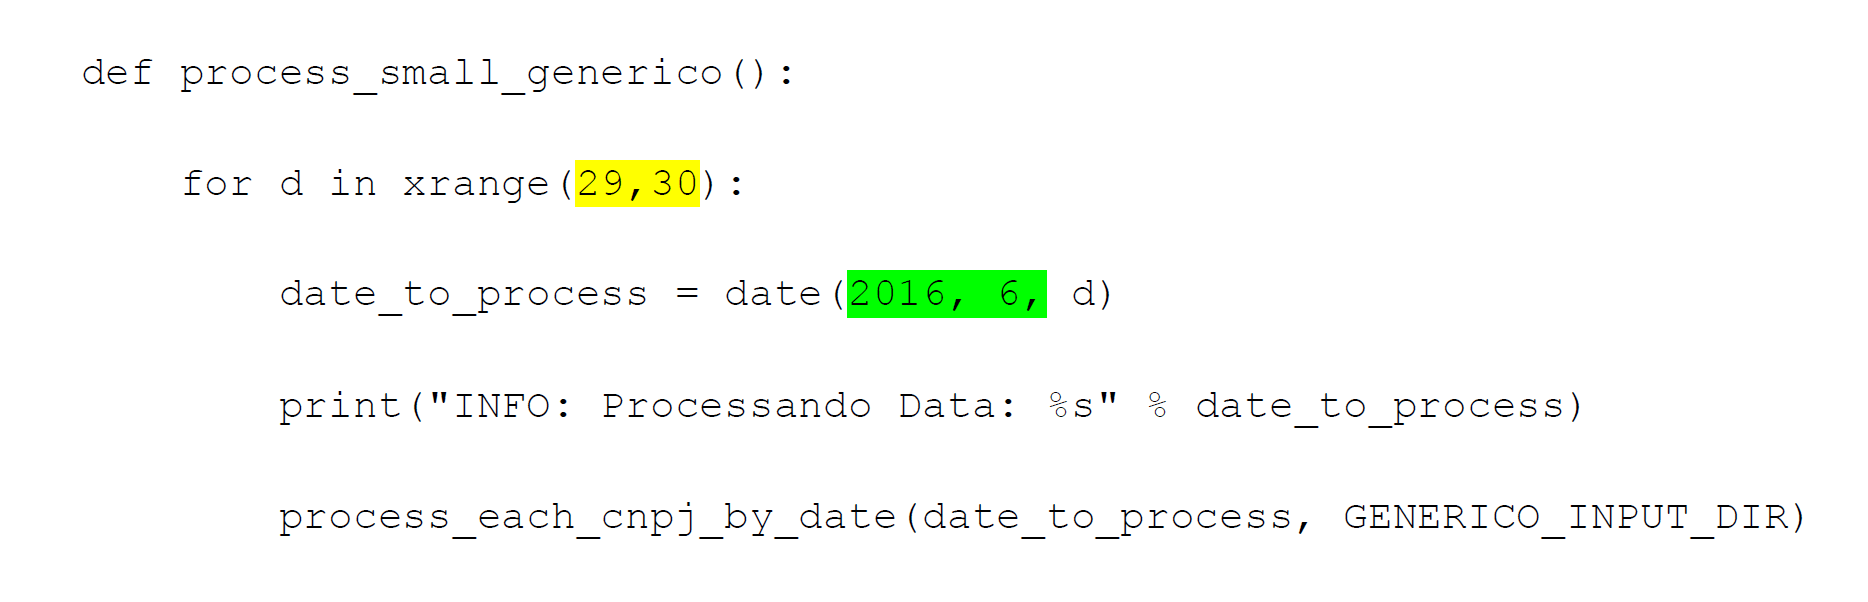
\includegraphics[width=1.0\textwidth]{genericos.png}
  \label{fig:genericos}
  \caption{Trecho de código a ser alterado}
\end{figure}

No exemplo da figura~\ref{fig:genericos} uma vez chamdo o $processa\_genericos.py$ pela linha de comando, processará \textbf{somente} o dia 29 do mês 6 de 2016.

Arquivos de logs com extensão \textbf{.log} serão gerados no mesmo diretório para auxiliar em caso de problemas.

O programa digere os dados da pasta \textbf{Cupons/processar (.NS)} e o resultado da digesão dos dados estarão na pasta \textbf{Cupons/processados (.csv, .pag).}



\section{Sugestão de testes}

\begin{itemize}
    \item Reprocessamento dos cupons Epson. Com especial atenção para o COO incorreto que NÃO é bug do digester.
    \item Reprocessamento de cupons Sweda.
\end{itemize}

\end{document}               % End of document.